\documentclass[aspectratio=169,14pt]{beamer}
\usetheme{default}\usecolortheme{default}\setbeamertemplate{navigation symbols}{}
\setbeamertemplate{footline}{\hfill{\scriptsize\color{covermuted}\insertframenumber/\inserttotalframenumber}\hspace{0.4cm}\vspace{0.15cm}}
\usepackage{fontspec}\usepackage{xeCJK}\setCJKmainfont{PingFang SC}[BoldFont=PingFang SC Semibold]\setmainfont{Helvetica Neue}[BoldFont=Helvetica Neue Bold]
\usepackage{xcolor}\usepackage{tikz}\usepackage{graphicx}\usepackage{fontawesome5}\usetikzlibrary{positioning,calc,arrows.meta,shadows}
\definecolor{bgmain}{RGB}{238,243,252}\definecolor{panel}{RGB}{238,244,255}\definecolor{factbg}{RGB}{246,242,235}\definecolor{coverprimary}{HTML}{2563EB}\definecolor{coveraccent}{HTML}{00A884}\definecolor{coverwarning}{HTML}{F59E0B}\definecolor{coverdark}{HTML}{1F2937}\definecolor{covermuted}{HTML}{64748B}\definecolor{titlecolor}{RGB}{30,30,30}\definecolor{muteddark}{RGB}{72,86,115}\definecolor{bluepanel}{RGB}{226,237,255}\definecolor{greenpanel}{RGB}{225,246,237}\definecolor{amberpanel}{RGB}{255,244,222}\definecolor{purplepanel}{RGB}{239,231,255}\setbeamercolor{background canvas}{bg=bgmain}
\newcommand{\plainbar}{\begin{tikzpicture}[remember picture, overlay]\fill[coverdark, opacity=0.07] (current page.south west) rectangle ([yshift=0.4cm]current page.south east);\draw[coveraccent, opacity=0.45, line width=0.8pt] ([yshift=0.4cm]current page.south west) -- ([yshift=0.4cm]current page.south east);\end{tikzpicture}}
\newcommand{\deckbackground}{\begin{tikzpicture}[remember picture, overlay]\fill[coverprimary!8] (current page.north west) rectangle (current page.south east);\fill[coverprimary!14] (current page.north west) ++(1.55,-1.35) circle (2.45cm);\fill[coveraccent!12] (current page.south east) ++(-1.9,1.45) circle (2.70cm);\fill[coverwarning!12] (current page.north east) ++(-2.9,-1.8) circle (0.85cm);\foreach \x in {-0.2,0.8,...,16.2} {\draw[coverprimary, opacity=0.045, line width=0.25pt] ([xshift=\x cm]current page.south west) -- ([xshift=\x cm]current page.north west);}\foreach \y in {-0.2,0.7,...,9.3} {\draw[coverprimary, opacity=0.04, line width=0.25pt] ([yshift=\y cm]current page.south west) -- ([yshift=\y cm]current page.south east);}\draw[coveraccent, opacity=0.38, line width=1.1pt] ([xshift=0.35cm,yshift=7.72cm]current page.south west) -- ++(3.25,0) -- ++(0.45,-0.45) -- ++(2.0,0);\draw[coverprimary, opacity=0.24, line width=1.0pt] ([xshift=9.35cm,yshift=8.25cm]current page.south west) -- ++(2.3,0) -- ++(0.55,-0.55) -- ++(3.2,0);\fill[coverdark, opacity=0.07] (current page.south west) rectangle ([yshift=0.42cm]current page.south east);\end{tikzpicture}}
\newcommand{\sectiontitle}[2]{\vspace{-0.52cm}\begin{center}{\fontsize{20}{24}\selectfont\bfseries\color{titlecolor} #1}\\[2pt]{\fontsize{9}{11}\selectfont\itshape\color{muteddark} #2}\end{center}\vspace{0.12cm}}
\newcommand{\portraitbox}[2]{\begin{tikzpicture}\node[draw=coverprimary!28, line width=0.7pt, fill=white, rounded corners=3pt, inner sep=2.5pt, drop shadow={shadow xshift=0.5pt, shadow yshift=-0.5pt, opacity=0.12}] {\includegraphics[width=2.4cm,height=2.9cm,keepaspectratio]{#1}};\end{tikzpicture}{\par\vspace{1pt}\fontsize{6.5}{7.5}\selectfont\color{covermuted} #2\par}}
\newcommand{\placeholderportrait}[2]{\begin{tikzpicture}\node[draw=coverprimary!28, line width=0.7pt, fill=white, rounded corners=3pt, inner sep=2.5pt, drop shadow={shadow xshift=0.5pt, shadow yshift=-0.5pt, opacity=0.12}] {\begin{tikzpicture}\fill[bluepanel] (0,0) rectangle (2.4,2.9);\foreach \x/\y in {0.25/0.45,0.55/1.85,0.95/1.15,1.35/2.2,1.75/0.85,2.1/1.65} {\fill[coverprimary!32] (\x,\y) circle (0.055cm);}\draw[coveraccent!45, line width=0.55pt] (0.25,0.45) -- (0.55,1.85) -- (0.95,1.15) -- (1.35,2.2) -- (1.75,0.85) -- (2.1,1.65);\node[circle, fill=coverprimary!16, minimum size=0.78cm] at (1.2,1.78) {};\node[rounded corners=8pt, fill=coverprimary!16, minimum width=1.28cm, minimum height=0.72cm] at (1.2,0.78) {};\node[font=\fontsize{12}{14}\selectfont\bfseries, text=coverprimary!75!black] at (1.2,0.17) {#1};\end{tikzpicture}};\end{tikzpicture}{\par\vspace{1pt}\fontsize{6.5}{7.5}\selectfont\color{covermuted} #2\par}}
\newcommand{\personslide}[9]{\begin{frame}\plainbar\vspace{-0.45cm}\begin{center}{\fontsize{22}{26}\selectfont\bfseries\color{coverdark} #1}\\[2pt]{\fontsize{9.5}{11.5}\selectfont\color{muteddark} #2}\end{center}\vspace{0.15cm}\begin{columns}[c]\begin{column}{0.22\textwidth}\centering #3\end{column}\begin{column}{0.28\textwidth}\begin{tikzpicture}\node[fill=greenpanel, rounded corners=4pt, inner xsep=6pt, inner ysep=5pt, text width=3.8cm, align=left] {{\fontsize{7}{8.5}\selectfont\bfseries\color{coveraccent!70!black} 获奖}\enspace{\fontsize{7}{8.5}\selectfont\color{coverdark!85} #4}\\[2.5pt]{\fontsize{7}{8.5}\selectfont\bfseries\color{coveraccent!70!black} 生卒}\enspace{\fontsize{7}{8.5}\selectfont\color{coverdark!85} #5}\\[2.5pt]{\fontsize{7}{8.5}\selectfont\bfseries\color{coveraccent!70!black} 身份}\enspace{\fontsize{7}{8.5}\selectfont\color{coverdark!85} #6}\\[2.5pt]{\fontsize{7}{8.5}\selectfont\bfseries\color{coveraccent!70!black} 机构}\enspace{\fontsize{7}{8.5}\selectfont\color{coverdark!85} #7}};\end{tikzpicture}\end{column}\begin{column}{0.48\textwidth}\begin{tikzpicture}\node[draw=coverprimary!35, fill=bluepanel, rounded corners=5pt, inner sep=7pt, text width=6.6cm, anchor=north west] at (0,0) {{\fontsize{8.6}{10.2}\selectfont\bfseries\color{coverprimary!82!black} 核心贡献}\\[3pt]{\fontsize{7.4}{9.2}\selectfont\color{coverdark!84} #8\\[3pt]\textbf{一句话：} #9}};\end{tikzpicture}\end{column}\end{columns}\end{frame}}
\begin{document}
\begin{frame}[plain]
\deckbackground
\begin{tikzpicture}[remember picture, overlay]
  \node[anchor=center, font=\fontsize{28}{34}\selectfont\bfseries, text=coverdark] at ([yshift=2.05cm]current page.center) {沃尔夫数学奖人物谱系};
  \node[anchor=center, font=\fontsize{15}{19}\selectfont, text=coverprimary!82!black] at ([yshift=0.86cm]current page.center) {第6集 \enspace·\enspace 拓扑革命};
  \node[anchor=center, font=\fontsize{12}{16}\selectfont\bfseries, text=coveraccent!76!black] at ([yshift=0.10cm]current page.center) {Topology · K-Theory · Manifolds · Gauge Theory};
  \draw[coveraccent, line width=1.4pt] ([yshift=-1.02cm, xshift=-4.55cm]current page.center) -- ([yshift=-1.02cm, xshift=4.55cm]current page.center);
  \node[anchor=center] at ([yshift=-1.90cm]current page.center) {\begin{tikzpicture}\node[rounded corners=8pt, fill=coverprimary!10, inner sep=4pt, minimum height=1.2em, font=\scriptsize\bfseries, text=coverprimary!85!black] at (-5.30,0) {Whitney};\node[rounded corners=8pt, fill=coverprimary!10, inner sep=4pt, minimum height=1.2em, font=\scriptsize\bfseries, text=coverprimary!85!black] at (-3.79,0) {Hirzebruch};\node[rounded corners=8pt, fill=coverprimary!10, inner sep=4pt, minimum height=1.2em, font=\scriptsize\bfseries, text=coverprimary!85!black] at (-2.27,0) {Milnor};\node[rounded corners=8pt, fill=coverprimary!10, inner sep=4pt, minimum height=1.2em, font=\scriptsize\bfseries, text=coverprimary!85!black] at (-0.76,0) {Bott};\node[rounded corners=8pt, fill=coverprimary!10, inner sep=4pt, minimum height=1.2em, font=\scriptsize\bfseries, text=coverprimary!85!black] at (0.76,0) {Sullivan};\node[rounded corners=8pt, fill=coverprimary!10, inner sep=4pt, minimum height=1.2em, font=\scriptsize\bfseries, text=coverprimary!85!black] at (2.27,0) {Novikov};\node[rounded corners=8pt, fill=coverprimary!10, inner sep=4pt, minimum height=1.2em, font=\scriptsize\bfseries, text=coverprimary!85!black] at (3.79,0) {Smale};\node[rounded corners=8pt, fill=coverprimary!10, inner sep=4pt, minimum height=1.2em, font=\scriptsize\bfseries, text=coverprimary!85!black] at (5.30,0) {Donaldson};\end{tikzpicture}};
\end{tikzpicture}
\end{frame}
\begin{frame}\plainbar\sectiontitle{拓扑革命}{Topology · K-Theory · Manifolds · Gauge Theory}\begin{center}\begin{tikzpicture}
  \node[draw=coverprimary!45, fill=bluepanel, rounded corners=5pt, inner sep=8pt, text width=11.2cm, align=left] at (0,1.05) {{\fontsize{8.3}{10}\selectfont\bfseries\color{coverprimary!80!black} 本集主线}\\[3pt]{\fontsize{7.4}{9.2}\selectfont\color{coverdark!84} 本集从微分拓扑、K 理论和 Bott 周期性讲到有理同伦、四维流形、规范理论和庞加莱猜想相关主线，展示拓扑如何改变 20 世纪数学的空间观。}};
  \node[draw=coverwarning!60, fill=amberpanel, rounded corners=5pt, inner sep=7pt, text width=11.2cm, align=center] at (0,-1.45) {{\fontsize{8.0}{9.8}\selectfont\bfseries\color{coverwarning!62!black} 开场问题}\\[-1pt]{\fontsize{7.4}{9}\selectfont\color{coverdark!82} 形状的本质是什么？为什么高维空间、四维流形和规范场会成为同一条拓扑主线？}};
\end{tikzpicture}\end{center}\end{frame}
\begin{frame}\plainbar\sectiontitle{人物路线图}{从早期奠基到现代前沿}\begin{center}\begin{tikzpicture}[milestone/.style={draw=coverprimary!45, fill=panel, rounded corners=4pt, inner xsep=4.0pt, inner ysep=5pt, align=center, font=\fontsize{5.7}{7.0}\selectfont\bfseries}, arrow/.style={-{Stealth}, draw=coveraccent, line width=0.7pt}]
\node[milestone, fill=bluepanel] (m0) at (-5.50,1.0) {1982\\Whitney};
\node[milestone, fill=greenpanel] (m1) at (-3.93,1.0) {1988\\Hirzebruch};
\draw[arrow] (m0) -- (m1);
\node[milestone, fill=amberpanel] (m2) at (-2.36,1.0) {1989\\Milnor};
\draw[arrow] (m1) -- (m2);
\node[milestone, fill=purplepanel] (m3) at (-0.79,1.0) {2000\\Bott};
\draw[arrow] (m2) -- (m3);
\node[milestone, fill=bluepanel] (m4) at (0.79,1.0) {2010\\Sullivan};
\draw[arrow] (m3) -- (m4);
\node[milestone, fill=greenpanel] (m5) at (2.36,1.0) {2005\\Novikov};
\draw[arrow] (m4) -- (m5);
\node[milestone, fill=amberpanel] (m6) at (3.93,1.0) {2006/07\\Smale};
\draw[arrow] (m5) -- (m6);
\node[milestone, fill=purplepanel] (m7) at (5.50,1.0) {2020\\Donaldson};
\draw[arrow] (m6) -- (m7);
  \node[draw=coverprimary!38, fill=white, rounded corners=5pt, inner sep=7pt, text width=11.4cm, align=left] at (0,-1.25) {{\fontsize{8.0}{9.8}\selectfont\bfseries\color{coverprimary!80!black} 叙事线}\\[-1pt]{\fontsize{7.2}{8.8}\selectfont\color{coverdark!82} 本集从微分拓扑、K 理论和 Bott 周期性讲到有理同伦、四维流形、规范理论和庞加莱猜想相关主线，展示拓扑如何改变 20 世纪数学的空间观。}};
\end{tikzpicture}\end{center}\end{frame}
\begin{frame}\plainbar\sectiontitle{本集的四个关键词}{观众需要记住的结构性线索}\begin{columns}[T]
\begin{column}{0.49\textwidth}\begin{tikzpicture}
\node[draw=coverprimary!45, fill=bluepanel, rounded corners=5pt, inner sep=7pt, text width=6.0cm, anchor=north west] at (0,0) {{\fontsize{8.5}{10}\selectfont\bfseries\color{coverprimary!80!black} 1. 流形}\\[2pt]{\fontsize{7.3}{8.8}\selectfont\color{coverdark!82} 把连续空间局部看成欧氏空间，再用全局不变量识别它们。}};
\node[draw=coverprimary!45, fill=greenpanel, rounded corners=5pt, inner sep=7pt, text width=6.0cm, anchor=north west] at (0,-2.25) {{\fontsize{8.5}{10}\selectfont\bfseries\color{coveraccent!70!black} 2. K 理论}\\[2pt]{\fontsize{7.3}{8.8}\selectfont\color{coverdark!82} 用向量丛和稳定等价提炼空间的深层代数结构。}};
\end{tikzpicture}\end{column}
\begin{column}{0.49\textwidth}\begin{tikzpicture}
\node[draw=coverprimary!45, fill=amberpanel, rounded corners=5pt, inner sep=7pt, text width=6.0cm, anchor=north west] at (0,0) {{\fontsize{8.5}{10}\selectfont\bfseries\color{coverwarning!62!black} 3. 同伦与动力}\\[2pt]{\fontsize{7.3}{8.8}\selectfont\color{coverdark!82} 空间的变形、映射和动力系统共同构成现代拓扑语言。}};
\node[draw=coverprimary!45, fill=purplepanel, rounded corners=5pt, inner sep=7pt, text width=6.0cm, anchor=north west] at (0,-2.25) {{\fontsize{8.5}{10}\selectfont\bfseries\color{coverprimary!74!black} 4. 四维与规范}\\[2pt]{\fontsize{7.3}{8.8}\selectfont\color{coverdark!82} 四维流形显示出异常精细的结构，规范理论成为突破工具。}};
\end{tikzpicture}\end{column}\end{columns}\end{frame}
\personslide
  {Hassler Whitney}
  {哈斯勒·惠特尼：微分拓扑的奠基者}
  {\portraitbox{images/Whitney.jpg}{Photo: Wikipedia}}
  {1982（74岁）}
  {1907--1989}
  {美国}
  {Institute for Advanced Study}
  {Whitney 在微分拓扑、奇点理论、图论和拟阵理论中贡献奠基，Whitney 嵌入定理和浸入理论成为流形研究的基本工具。}
  {他让“光滑流形如何放进欧氏空间”成为可精确处理的问题。}
\personslide
  {Friedrich Hirzebruch}
  {弗里德里希·希策布鲁赫：拓扑、代数几何与战后德国数学}
  {\portraitbox{images/Hirzebruch.jpeg}{Photo: Wikipedia}}
  {1988（60岁）}
  {1927--2012}
  {西德}
  {University of Bonn / Max Planck Institute}
  {Hirzebruch 证明 Hirzebruch-Riemann-Roch 定理，连接拓扑、代数几何和特征类，并推动波恩成为战后欧洲数学中心。}
  {他把特征类、指标和代数几何放进同一张地图。}
\personslide
  {John Milnor}
  {约翰·米尔诺：异国球面与微分拓扑}
  {\portraitbox{images/Milnor.jpg}{Photo: Wikipedia}}
  {1989（58岁）}
  {1931--}
  {美国}
  {SUNY Stony Brook}
  {Milnor 发现异国球面，在微分拓扑、K 理论和动力系统中均有深远贡献；他同时获得菲尔兹奖和阿贝尔奖。}
  {他证明同一个拓扑球面可以拥有不同的光滑结构。}
\personslide
  {Raoul Bott}
  {劳尔·博特：Bott 周期性}
  {\portraitbox{images/Bott.jpg}{Photo: Wikipedia}}
  {2000（76岁）}
  {1923--2005}
  {匈牙利/美国}
  {Harvard University}
  {Bott 周期性定理深刻影响 K 理论、同伦论、指标理论和规范理论，是现代拓扑的核心定理之一。}
  {他揭示了拓扑不变量背后的周期节奏。}
\personslide
  {Dennis Sullivan}
  {丹尼斯·沙利文：有理同伦与拓扑动力}
  {\portraitbox{images/Sullivan.jpg}{Photo: Wikipedia}}
  {2010（69岁）}
  {1941--}
  {美国}
  {SUNY Stony Brook / CUNY}
  {Sullivan 在拓扑、动力系统、有理同伦论、叶状结构和复动力系统中贡献核心；2022 年获阿贝尔奖。}
  {他把拓扑的柔性方法带入动力系统和几何结构。}
\personslide
  {Sergei Novikov}
  {谢尔盖·诺维科夫：Pontryagin 类与高维拓扑}
  {\portraitbox{images/Novikov.jpg}{Photo: Wolf Foundation}}
  {2005（67岁）}
  {1938--2024}
  {俄罗斯}
  {University of Maryland / Landau Institute}
  {Novikov 在拓扑、Pontryagin 类、同伦论和孤立子理论中贡献深远，是菲尔兹奖得主。}
  {他让高维流形的不变量进入现代拓扑核心。}
\personslide
  {Stephen Smale}
  {斯蒂芬·斯梅尔：庞加莱猜想、高维拓扑与动力系统}
  {\portraitbox{images/Smale.jpg}{Photo: Wikipedia}}
  {2006/07（76岁）}
  {1930--}
  {美国}
  {UC Berkeley / Toyota Tech / City Univ. of HK}
  {Smale 证明高维庞加莱猜想，在微分拓扑、动力系统、经济学数学和数值分析中影响巨大；1966 年获菲尔兹奖。}
  {他把拓扑和动力系统都推向了现代形态。}
\personslide
  {Simon Donaldson}
  {西蒙·唐纳森：四维流形与规范理论}
  {\portraitbox{images/Donaldson.jpg}{Photo: Wikipedia}}
  {2020（62岁）}
  {1957--}
  {英国}
  {Imperial College London / SUNY Stony Brook}
  {Donaldson 用 Yang-Mills 规范理论研究四维光滑流形，发现四维拓扑的特殊复杂性；1986 年获菲尔兹奖。}
  {他把物理中的规范场变成四维拓扑的显微镜。}
\begin{frame}\plainbar\sectiontitle{第6集的主线}{拓扑革命}\begin{center}\begin{tikzpicture}[block/.style={draw=coverprimary!42, fill=white, rounded corners=5pt, inner sep=6pt, text width=3.0cm, align=center, font=\fontsize{7.0}{8.5}\selectfont}, arrow/.style={->, draw=coveraccent, line width=0.85pt}]
  \node[block, fill=bluepanel] (a) at (-4.9,1.25) {\textbf{起点}\\基础语言}; \node[block, fill=greenpanel] (b) at (-1.65,1.25) {\textbf{工具}\\结构方法}; \node[block, fill=amberpanel] (c) at (1.65,1.25) {\textbf{突破}\\核心定理}; \node[block, fill=purplepanel] (d) at (4.9,1.25) {\textbf{影响}\\跨域应用};
  \draw[arrow] (a) -- (b); \draw[arrow] (b) -- (c); \draw[arrow] (c) -- (d);
  \node[draw=coverwarning!65, fill=factbg, rounded corners=5pt, inner sep=7pt, text width=11.1cm, align=left] at (0,-1.35) {{\fontsize{8.0}{9.8}\selectfont\bfseries\color{coverwarning!62!black} 一句话总结}\\[-1pt]{\fontsize{7.4}{9}\selectfont\color{coverdark!84} 本集从微分拓扑、K 理论和 Bott 周期性讲到有理同伦、四维流形、规范理论和庞加莱猜想相关主线，展示拓扑如何改变 20 世纪数学的空间观。}};
\end{tikzpicture}\end{center}\end{frame}
\begin{frame}\plainbar\sectiontitle{下一步}{专题系列衔接}\begin{center}\begin{tikzpicture}
  \node[draw=coverwarning!60, fill=coverwarning!12, rounded corners=5pt, inner sep=7pt, text width=10.5cm, align=center] at (0,1.4) {{\fontsize{8.4}{10}\selectfont\bfseries\color{coverwarning!65!black} 下一集：微分几何、几何分析与辛几何}\\[-1pt]{\fontsize{7.4}{9}\selectfont\color{coverdark!80} 继续沿着沃尔夫奖人物谱系，进入下一条数学主线。}};
  \node[draw=coverprimary!45, fill=bluepanel, rounded corners=5pt, inner sep=8pt, text width=10.5cm, align=center] at (0,-1.35) {{\fontsize{10.5}{12.8}\selectfont\bfseries\color{coverprimary!82!black} Chern、De Giorgi、Gromov、Yau、Mostow、Schoen、Eliashberg}};
\end{tikzpicture}\end{center}\end{frame}
\end{document}
